\chapter{REVIEW OF DATA VISUALIZATION AND DELIVERY TECHNIQUES}
\label{chap:intro}

The advent of big data sets has put pressure on the Mathematics and Statistics community to rethink how to apply traditional of analysis and inferencing. Both climate and oceanographic science disciplines are feeling this data explosion and are struggling to scale. Unprecedented amounts of data are made available by governmental agencies like \gls{noaa} and \gls{nasa}, and heavily used by the scientific community to draw inferences. The traditional visualization and delivery tools can be improved to handle a surge of new data delivery. The techniques used to visualize and retrieve these data needs to be reevaluated. Global predictions need modern web app technologies for professional and amateur to visualize and receive data quickly, accurately, and as painlessly as possible.

Traditional methods of parsing through a remote/local archive of files, selecting relevant files, opening the files and performing analysis on a single pc do not scale with big data. Scientists are spending more time navigating through data rather than finding discoveries. Worse still, amateurs in the form of young people, hobbyists, students and potential scientists get frustrated and give up on using these rich data sets. Toolkits and web apps are suggested in this thesis to relieve this pressure. Modern \gls{restfull} app design gives the community a walking stick to help them wade through the big data mire.

It's worth mentioning here another big data paradigm. Distributed systems/cloud computing offers the scientific community a means to handle big data at the expense of complicated overhead and expensive cloud-based services, such as \gls{aws}. Most scientists do not want, or in many cases do not even need these services. They need a subset of big data, or to be able to break down a data set into smaller pieces for their studies. Cloud computing services do not address the issue of accessibility and visualization. Comparing toolkits/web apps to cloud platforms are not opposing viewpoints. Instead, they can be used (or not) to varying degrees.

An unsettling reality is that as new technologies unfurl, mathematicians, statisticians, and scientists are pressured to adopt them without question or complaint. Expecting the community to embrace new paradigms is impracticable, and branding scientists who are reluctant to embrace as 'old school' manifest the fallacy that new is better, young outpaces the old, and what you learned yesterday has no use today. This fallacy also cloaks the issue with these new paradigms: they are not needed for most scientific applications. In the context of the problem posed in this thesis, we are interested in big data visualization and delivery, and tailor this solution to what the community wants/needs. In this scope, big data is divided piecemeal into relevant sections that can be visualized and delivered with minimal domain expertise.

Time series analysis and gridded interpolation of climate systems are usually done on local spatiotemporal realms. The mathematical models that describe complex systems simplify climate regimes to seasonal, spatial, and temporal scales small enough to be computed on a single machine. A butterfly's flapping its wings in the Amazon is not modeled for Gulf rainfall after all! In this sense, the methods used to simplify the data is under investigation. Models are evaluated by how well they fit different data sets, and it is of interest to the community to try as many models as possible and to compare results with each other. In this sense, data visualization and accessibility aid the scientific process, as it allows ease of data for modeling, and is means of comparing. In the next sections, we hope to introduce current visualization platforms available for two different datasets. A 3D gridded satellite product, and a 4D in situ ocean sensor array product.

\section{INTERACTIVE MULTISENSOR SNOW AND ICE MAPPING SYSTEM DATA VISUALIZATION}

The daily snow and ice coverage dataset over the Northern Hemisphere (NH)
based on the Interactive Multisensor Snow and Ice Mapping System (IMS) maintained by the United States' NSIDC \cite{NIC} is a useful tool for numerous applications, such as monitoring day-to-day weather variations for water resources and agriculture, and estimating the snowstorm severity for insurance industries and governmental agencies. 
The IMS data derives from remote sensing of multiple satellites, including NOAA POLES satellites,
MODIS Aqua and Terra, as well as {\it in situ} observations. \cite{fetterer2011ims,ramsay1998interactive}
The dataset began on 4 February 1997 and has numerous users, ranging from professionals including climate scientists, satellite remote sensing experts, hydrological engineers to high school students and climate science enthusiasts. A few visualization sites cater to this broad audience, offering a quick visualization platform. 

Rutgers University Global Snow Lab provides a daily snow-cover \url{https://climate.rutgers.edu/snowcover/} \cite{rutgers_sl}. Here users can scroll through preprocessed images of the daily snow cover. Visualization is limited to scrolling through images. There are no zooming features, or time series offered.

The United States National Snow and Ice data center provide another image archive at \url{http://www.natice.noaa.gov/ims/} \cite{nat_ice}. Here users also can download images of IMS’s daily northern hemisphere snow and ice coverage. Additionally, they can view and download United States, Alaska, Europe/Asia, and Afghanistan regions. As with Rutgers site, the users are unable to zoom or download the actual data. Furthermore, the actual square coverage for this site is limited to pixels on an image. Estimating square km areas are limited to a 3-day mean ice coverage chart, showing maximum and minimum bars along with a dotted line average shown in Figure~\ref{fig:nat_ice}

\begin{figure}[ht]
  \centering
  \begin{minipage}{4.5in}
    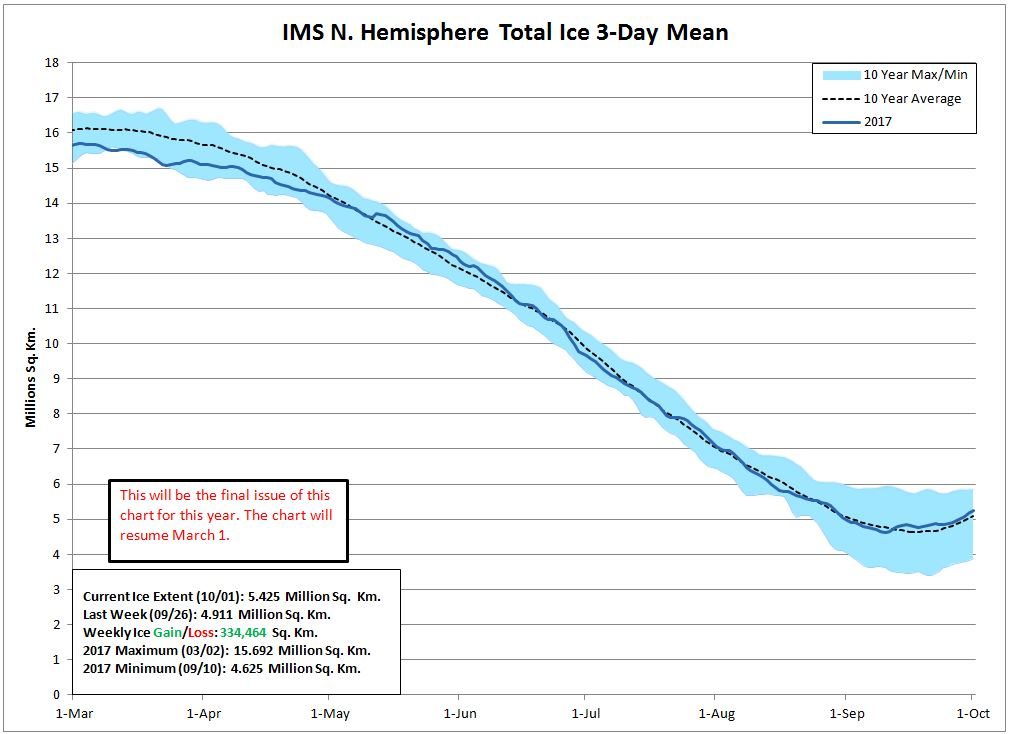
\includegraphics[width=\linewidth]{ims_data.jpg}
    \caption{ \label{fig:nat_ice} Sea and Lake Ice coverage of IMS data using 4 KM resolution. Ice coverages are calculated using a three day running mean from March until September each year. Blue border displays maximum and minimum values for the season. Areas are calculated using the Lambert Azimuthal Equal Area Projection with a WGS84 Datum. \cite{nat_ice}}
  \end{minipage}
\end{figure}

Users are left to examine two figures with square kilometers provided but are not able to see how the area is calculated. The IMS' calculation of the actual snow-covered area based on each grid box needs clarification. Because IMS provides images on a polar stereographic projection, the pixel area is a distortion of the true square kilometer coverage. Projecting a three-dimensional sphere/ellipsoid on a 2d plane using a stereographic projection stretches out low latitude areas and contracts high latitudes \cite{snyder1987map}. The IMS community would benefit to know how to make this calculation, or better still, have software calculates the true area for them.

Chapter 2 of this thesis describes a software toolkit written in Python that calculates areas of the coverage provided by the Northern hemisphere. This toolkit also parses through the IMS data set for a given latitude-longitude. This thesis shall provide the theoretical basis for the toolkit, along with a time series analysis of the Tibetan Plateau Area. This toolkit is used by the Institute of Tibetan Plateau Research Chinese Academy of Sciences to produce daily snow coverage images located at \url{http://www.tpedatabase.cn/tibetSnow.jsp} \cite{TP_database}. 

Information and improvements regarding the toolkit shall be discussed, chiefly the opportunity for the creation of a web application that provides users with visualization and data retrieval built with modern website technology. Providing the source code limits the users to those who know Python; on the other hand, a web app connected to an intuitively designed user interface is a pragmatic way to serve the current IMS community to expand its user base.

\section{ARGO VISUALIZATION AND DATA RETRIEVAL}

For over a decade, the Argo program has provided temperature, salinity and pressure data (T/S/P) on a global scale for depths as far as 2000 decibar (dbar), with unprecedented spatial and temporal resolution and no seasonal bias \cite{argo}. Close to two million profiles have been collected and made publicly available on Argo’s Global Data Assembly Centres (GDACs) on \gls{ftp} servers. Data is recorded by various types of floats that drift at a resting depth and raise every few days to transmit information to GDACS. From there data underwent quality control markers and adjustments and released as a \gls{NetCDF} product on FTP servers. Users can download either profile (one cycle of a floating measurement) or the entire profile history of a float. Though there are visualization tools available, almost all of them do not allow querying based on a spatial-temporal selection. For example, retrieving Argo profile data for North Sea regions at a certain depth and date. Chapter 3 will describe a web app that is used to allow such a data retrieval service.

\subsection{Profile Cycles for Floats}

Argo floats are equipped with an inflatable bladder, allowing them to float and sink. Once deployed the floats are programmed to drift at a 1000 meter depth for nine days. After nine days before descending to 2000 meters, then rising at a rate of 10 cm/s. While ascending the float sensors begin sampling parameters described in Table~\ref{tbl:argoParams}. Ascension takes 6 hours. Once at the surface the float transmits data via satellite to the GDAC, taking 6-12 hours for floats using the Argos1 and Argos2 satellite systems. \cite{argo_uk}.

As early as 2005, floats with GPS navigation have been introduced \cite{argo_man}. Iridium and Argos-3 satellite systems data transmitted in a matter of minutes. The ratio of ARGOS to GPS floats is displayed over time by Figure ~\ref{fig:commTS}, collected from the Argovis database. According to this plot, Argos makes up $\approx 36\%$ of all profiles released, and GPS makes up $\approx 64\%$. Not only is GPS faster, but also allows higher frequency sampling. Floats that use GPS transmit $\approx 1000$ samples for each parameter. In contrast, Argos1 and Argos2 transmits only $\approx 100$. The Argo dataset is growing as more floats are deployed \textit{and} with increased sampling rates.

\begin{figure}[ht]
  \centering
  \begin{minipage}{4.5in}
    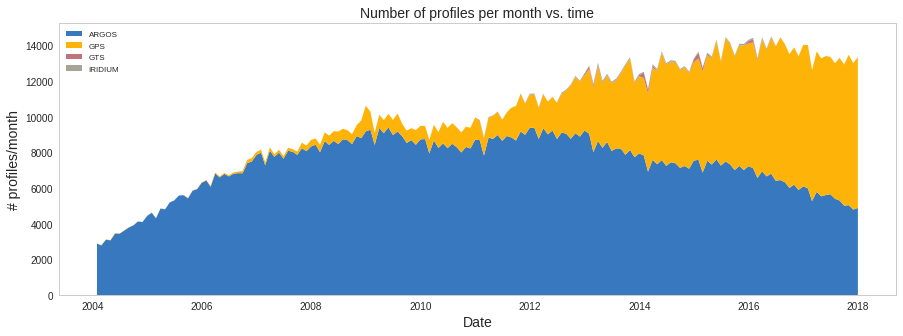
\includegraphics[width=\linewidth]{commTS.png}
    \caption{ \label{fig:commTS} Satalite Communication Type by month. Iridium floats also use the GPS system.}
  \end{minipage}
\end{figure}

\begin{figure}[ht]
  \centering
  \begin{minipage}{4.5in}
    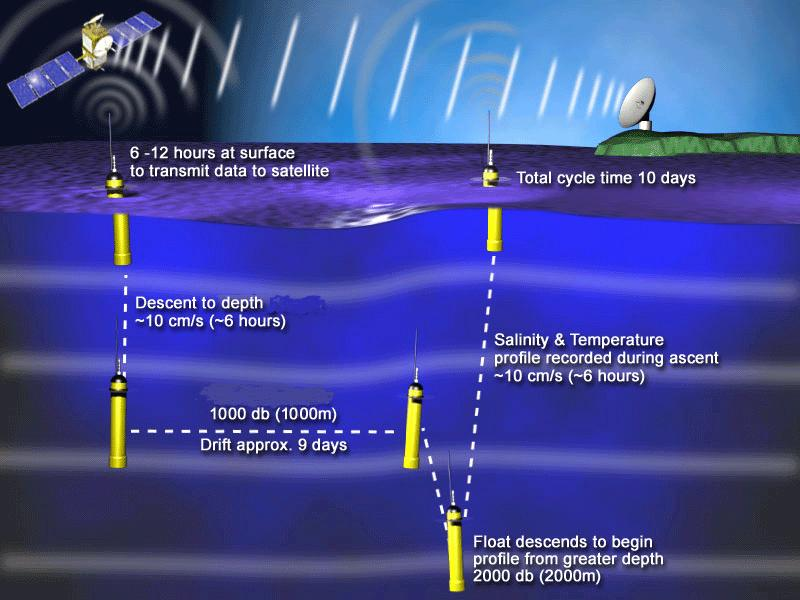
\includegraphics[width=\linewidth]{operation_park_profile.jpg}
    \caption{ \label{fig:argo_cycle} Detail of one profile cycle\cite{argo}}
  \end{minipage}
\end{figure}

\subsection{Float Hardware and Data Transmission}

An international program such as Argo consists of many float types for different functions. In addition to T/S/P, some floats optic/biologic measurements, as shown in table ~\ref{tbl:argoParams}

\begin{table}[th]
\caption{Abridged list of Argo mission parameters.}
\label{tbl:argoParams}
{\begin{tabular}{ | p{4.5cm} | p{5cm} | p{4cm} |} 
        \hline
        \textbf{Parameter name} & \textbf{long name} & \textbf{units} \tabularnewline \hline
        CNDC & conductivity & Siemens/m \tabularnewline \hline
        PRES & sea water pressure & decibar \tabularnewline \hline
        PSAL & practical salinity & practical salinity unit \newline (psu) \tabularnewline \hline
        TEMP & sea temperature & Celsius  \tabularnewline \hline
        DOXY & dissolved oxygen & $\mu Mol/kg$  \tabularnewline \hline
        BBPx & particle backscattering at x \newline nanometers & $1/m$  \tabularnewline \hline
        TURBIDITY & sea water turbidity & nephelometric turbidity \newline unit (NTU)  \tabularnewline \hline
        CPx & Particle beam attenuation at x \newline nanometers & $1/m$   \tabularnewline \hline
        CHLA & chlorophyll-A & $mg/m^3$   \tabularnewline \hline
        CDOM & concentration of coloured \newline dissolved organic matter in \newline sea water & ppb \tabularnewline \hline
        NITRATE & nitrates & $\mu Mol/kg$ \tabularnewline \hline
        BISULFIDE & bisulfides & $\mu Mol/kg$ \tabularnewline \hline
        PH\textunderscore IN\textunderscore SITU\textunderscore TOTAL & pH & dimensionless \tabularnewline \hline
        DOWN\textunderscore IRRADIANCEx & downwelling irradiance at \newline x nanometers & $W/m^2/nm$ \tabularnewline \hline
        UP\textunderscore IRRADIANCEx & upwelling irradiance at \newline x nanometers & $W/m^2/nm/sr$ \tabularnewline \hline
        DOWNWELLING\textunderscore PAR & downwelling photosynthetic \newline available radiation & $\mu Mol\ Quanta\ sec/m^2$ \tabularnewline \hline
        \end{tabular}}
\end{table}

\subsection{Data Delivery}

All Argo data collected since its inception is available at a US-based GDAC FTP server at \url{ftp://usgodae.org/pub/outgoing/argo/} or a Europian Server at \url{ftp://ftp.ifremer.fr/ifremer/argo/}. Users navigate through directory structure with sparse documentation. Each DAC folder contains float and profile netCDF files. From there users can either download netCDF, either individually or bundled together by its float. The server is designed for those familiar with the Argo manual \cite{argo_man}. Each float file is named by its WMO number. Each profile file is designated by its WMO number appended by the cycle number and prefixed with a real-time/delayed-time marker. The amount of data available to the user is on the scale of hundreds of Gigabytes, yet there is no way to select data based on location, date, measured parameters, etc. A few opportunities to allow better navigation arise if the Argo data is transferred to a database. By design, databases can be queried quickly by indexing frequently queried fields such as latitude, longitude, date, WMO, et cetera.

Databases are designed to accomplish storing and accessing large datasets. As Argo grows and expands, methods for reporting large and more complex data is essential to allow access to this information to as many people as possible. This database required to have an intuitive interface for selection, such as that made by the Coriolis group shown in Figure~\ref{fig:argo_france}. The next section introduces a proposed database and web-application interface.

\subsection{Argo Visualization Tools}

The limitations of selecting by profile and platform number through an FTP server has caused visualization tools to sprout up among the Argo community. The majority of these applications are based on visualization, and their utility is somewhat limited to displaying points on a map. A few prominent ones are mentioned below. Their merits and limitations shall be covered in detail before revealing the Argovis web app covered in Section~\ref{argovis} and Chapter 3.

\subsubsection{Coriolis Visualization Application} \label{coriolis}

Coriolis, Argo's French group, includes an app showing profiles on a tile map interface.\cite{argo_fr}. Users can pan, zoom in and out, and select floats on the map, represented by dots. See Figure \ref{fig:argo_france} for a screenshot of the webpage. Moreover, the site includes velocity fields derived from drifting floats provided via the ANDRO product \cite{ANDRO}. Data displayed on the map is limited to profiles reported within the past week. Upon clicking a point, a sidebar opens, revealing interactive charts of Pressure vs. Temperature and Pressure vs. Salinity. The side panel also includes meta-data: float identification number (WMO), date, DAC, project name, primary investigator and float model. Data can be viewed and downloaded in greater detail by clicking on links to another page.

\begin{figure}
\begin{minipage}{6in}
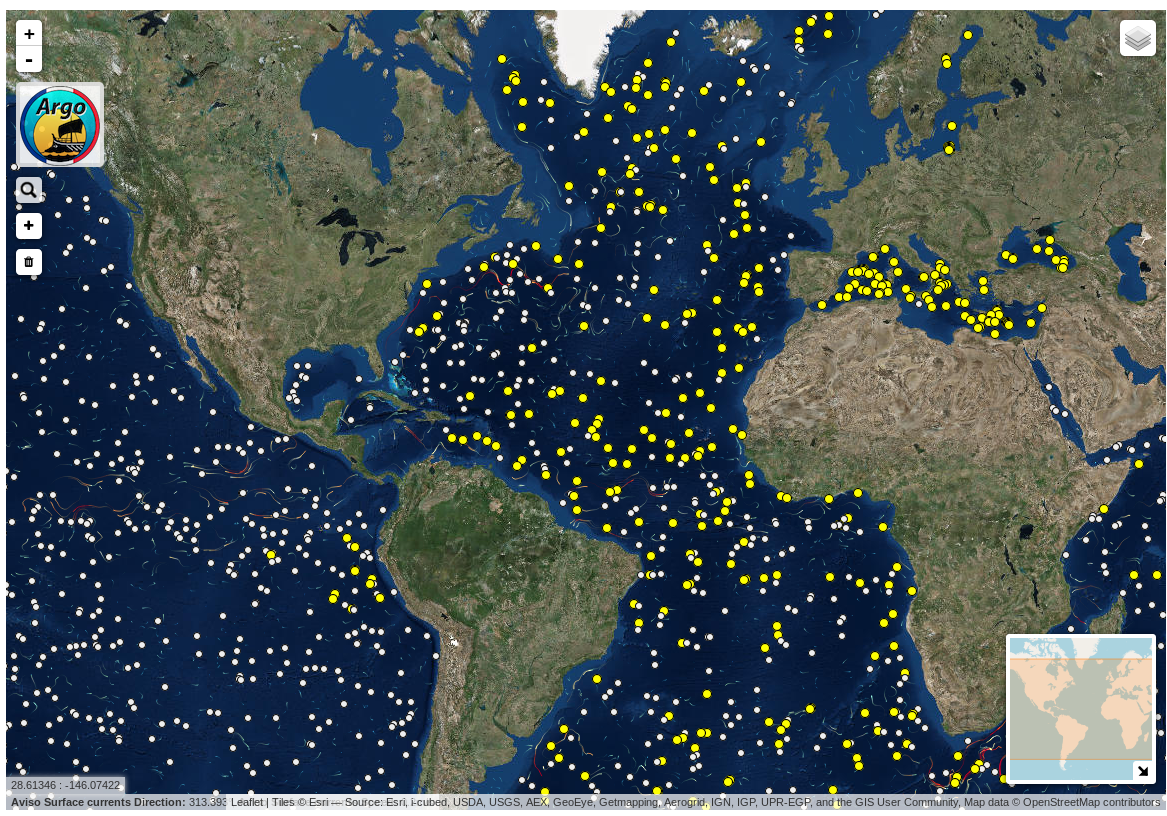
\includegraphics[width=.5\linewidth]{argo_france.png}
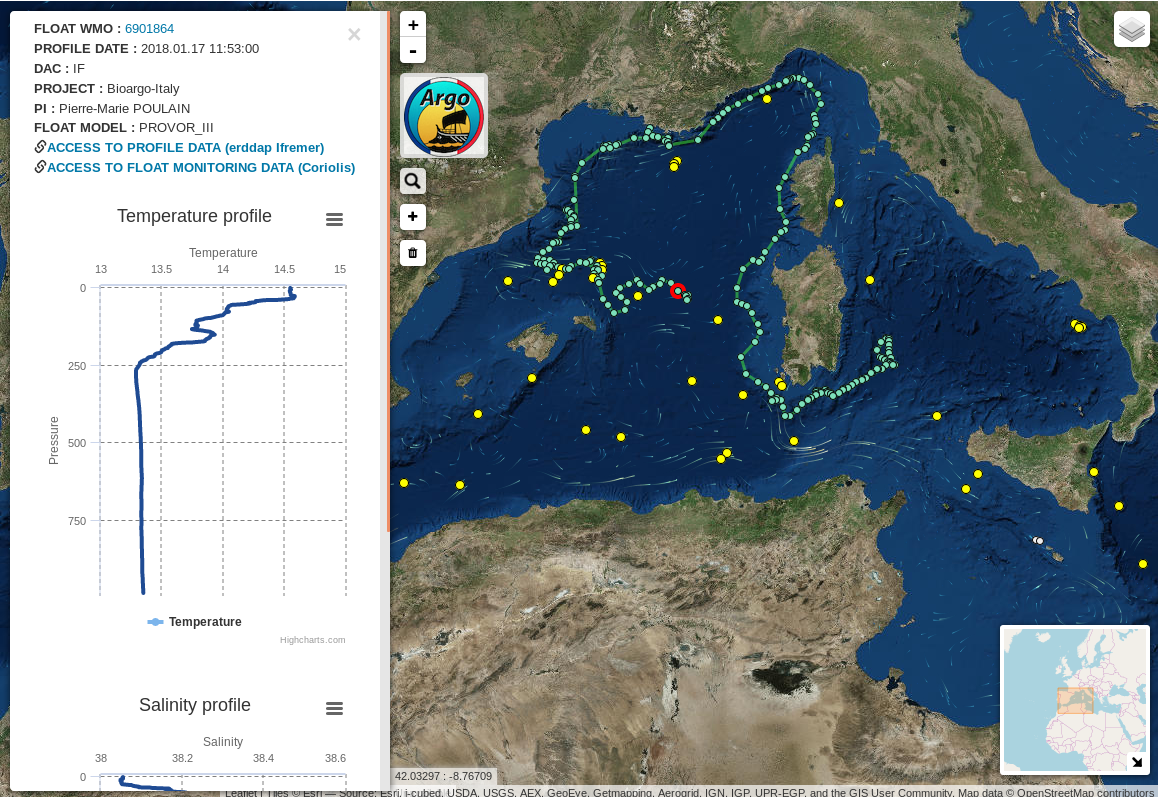
\includegraphics[width=.5\linewidth]{argo_france_zoomed.png}
\caption{\label{fig:argo_france}Argo Active network map (left) \url{http://www.argo-france.fr/en/argo-active-network-map/}\cite{argo_fr} Showing argo profiles owned by the Coriolis (French) DAC. Yellow dots represent floats operated by the Coriolis project. Selecting a dot reveals a side panel with additional information (right). Velocity field animations overlay the profile dots showing currents generated via ANDRO.}
\end{minipage}
\end{figure}

Argo-active-network-map's primary function is visualization but restrictive even at that. Users can only view one profile at a time for profiles reported in the last seven days. More importantly, they restricted from making spatial-temporal selections. Tilemap interfaces have draw plugins that allow users to draw polygon shapes. These points can then be used to select and view profiles contained within that polygon. It can be useful for users interested in climate change to view data on decadal timescales. Nonetheless, the app provided by Coriolis is a significant advancement over the main source of accessing Argo data on FTP server.

\subsubsection{NASA Sea Level Change Data Analysis Tool} \label{dat}

The \gls{dat} has been designed to allow for quick-look comparisons and analysis of NASA datasets of sea level change. The project is in its beta phase and can be viewed at \url{https://sealevel.nasa.gov/data-analysis-tool/}\cite{nasaSLR}. Gridded Argo products, among many other in situ and remote sensing products make up this app. The project states that its goal is to track sea level rise, it can visualize Argo temperature and salinity data. 

DAT comprises of interactive map and side control bar shown on ee Figure~\ref{fig:dat}. The mapping component uses an open source library \gls{cmc} library, located at \url{https://github.com/nasa/common-mapping-client}.

\begin{figure}
\begin{minipage}{6in}
\centering
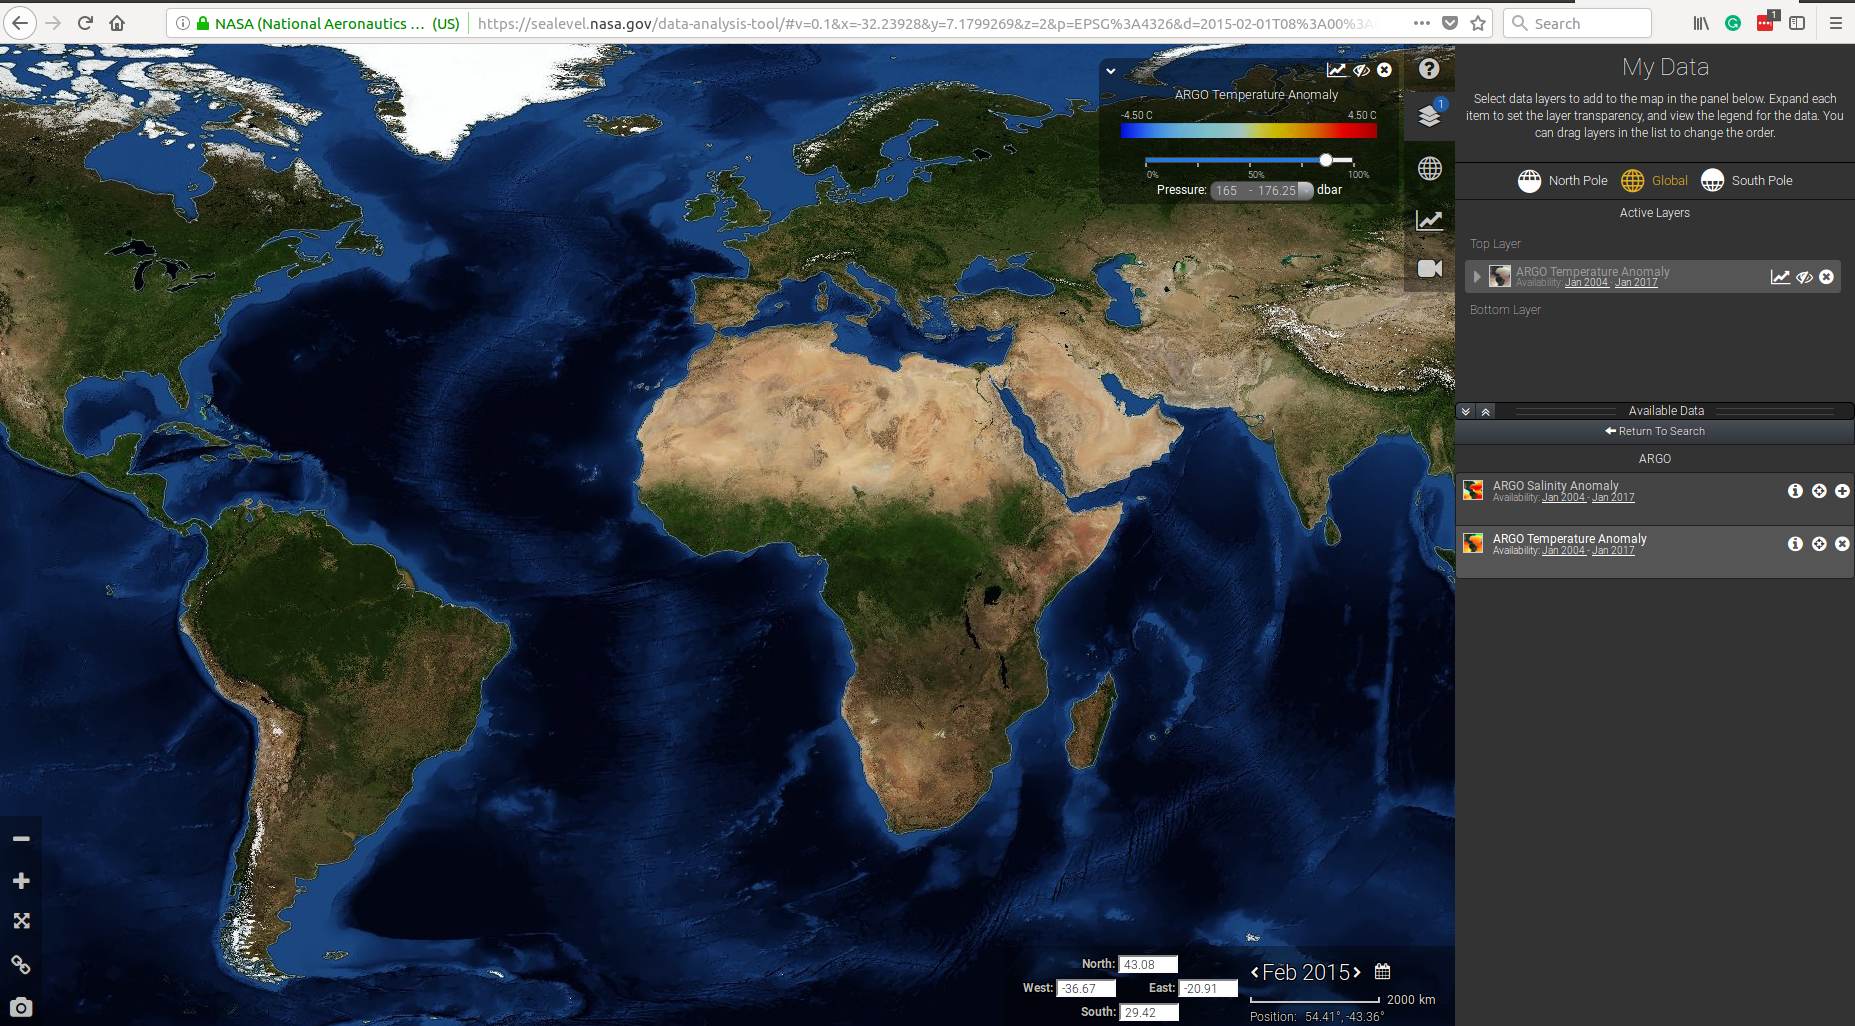
\includegraphics[width=\linewidth]{datMain.png}
\caption{\label{fig:dat} DAT web app format with Data tab displayed on the side bar. Argo derived gridded salinity and temperature products from January 2004 to January 2017 are available to plot.}
\end{minipage}
\end{figure}

CMC allows drawing points, lines and rectangles on the Mercator projection only. Lines vertically slice the ocean, whose temperature and salinity is viewed in a color chart. Shapes are editable, and plots are redrawn by clicking a new button. Unfortunately, this feature is not available for Argo data at this time.

Images of temperature and salinity overlay the CNC map. Users select which depth time, and an image of either temperature or salinity anomalies are displayed. See Figure~\ref{fig:dat_color_map}

\begin{figure}
\begin{minipage}{6in}
\centering
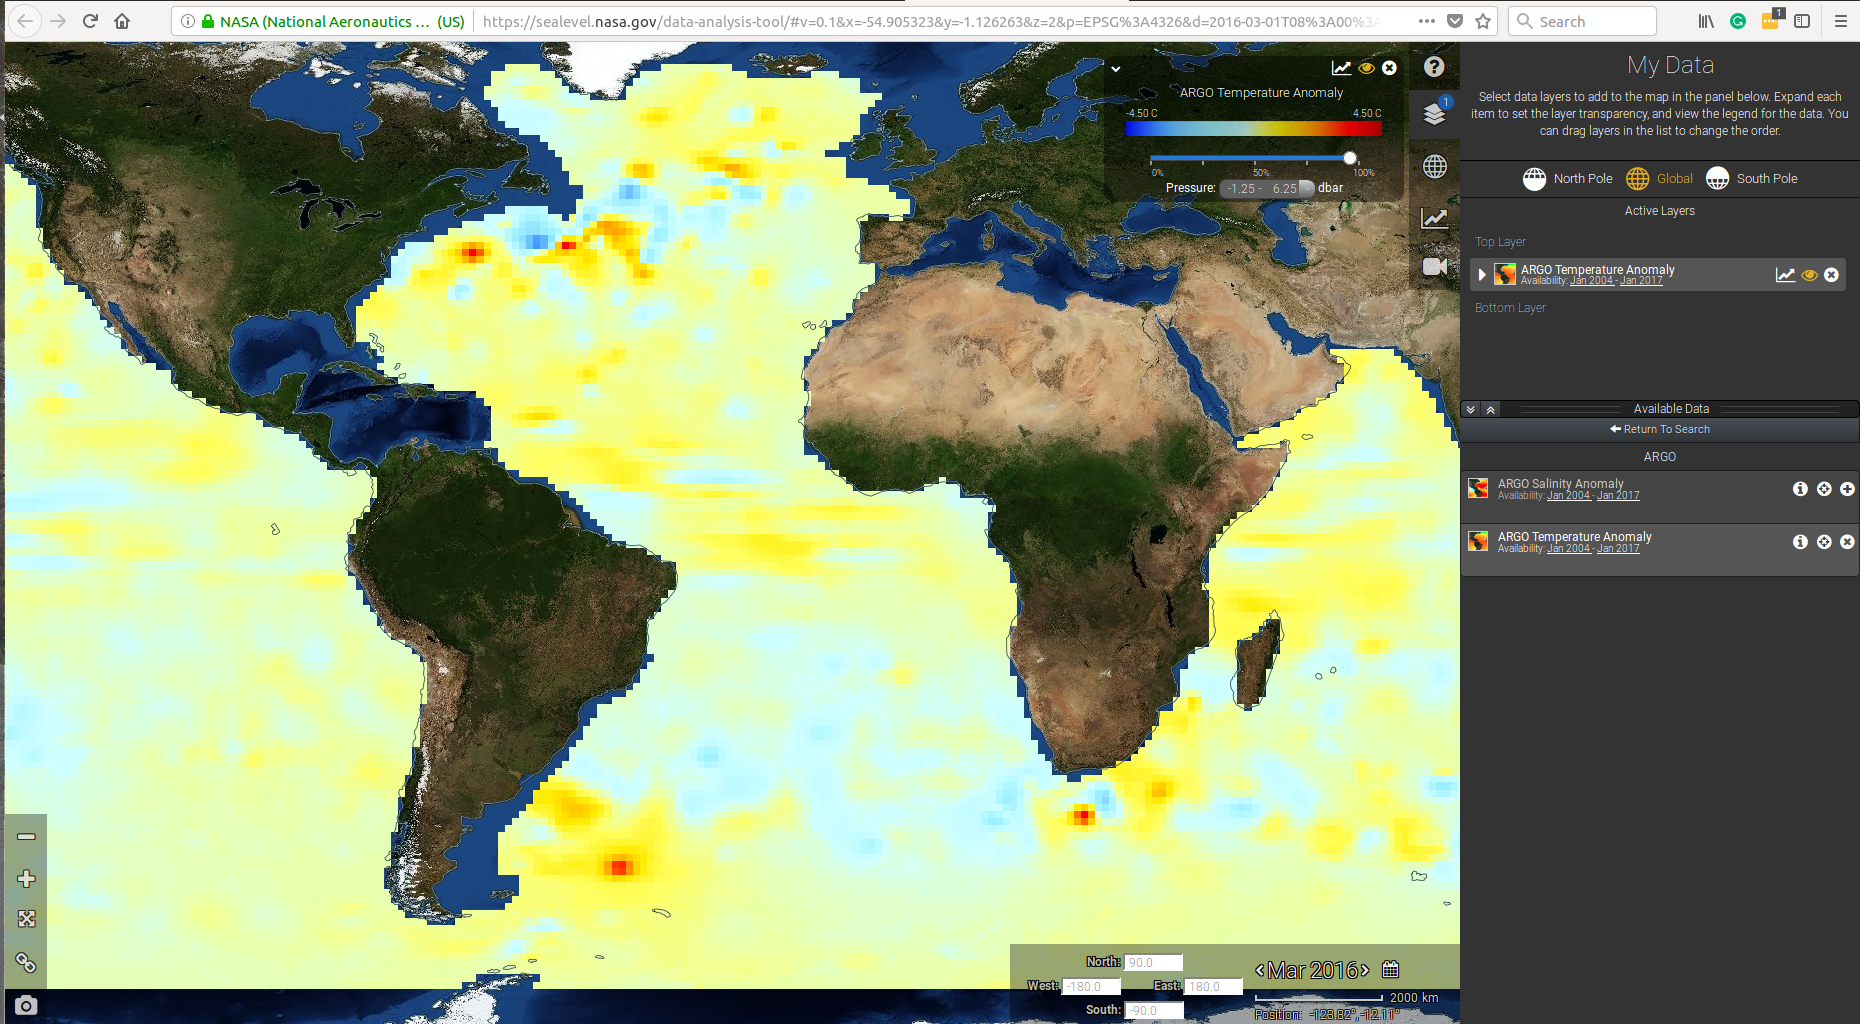
\includegraphics[width=\linewidth]{datTempAnom.png}
\caption{\label{fig:dat_color_map} DAT web app format with temperature anomalies layer displayed. Anomolies are for March 2016, indicated by the date selection on the bottom right. Pressure ranges are from -1.25 to 6.25 dbar, as indicated by the drop-down menu shown on the top right portion of the map.}
\end{minipage}
\end{figure}

Views and data are accessed through the URL. This RESTfull design extends the app beyond the browser. It allows API extensions data access without the need of the user manually retrieving data by a series of clicks on the browser. Scientists can automate these tasks for Repeatability and scalability.

DAT is an unprecedented tool in making selections from large climate data sets, yet some features limit its potential to be widely used by the Argo community.

\begin{enumerate}
\item The map cuts off at 180 degrees latitude. Unfortunately, the map cuts off in the middle of the Pacific basin. 
\item It is unclear how the gridded product interpolates Argo profiles. With no reference to the source, scientists are reluctant to use this data other than visualization.
\item The CMC library is capable of plotting points, yet Argo products are limited to gridded products. DAT would benefit from having a platform plotting feature, similar to the app covered in Section~\ref{coriolis}.
\item Does not allow images to show using different projections. South Sea and North Sea ocean views are limited. Stereographic projections would better serve these regions of interest. Storing data and plotting it using a heat map plugin displays the data in any map projection. 

\end{enumerate}

The app generates plots on the server-side. The client side doesn't get strained, making the app more responsive. The downside here is that the server requires more resources to work efficiently, making the app expensive to run and maintain.

This project sets a new precedence for data delivery and visualization. However, the cons may discourage its use as a scientific tool. In the later sections, these pros and cons are addressed. A compromise attempted that balances visualization features with data transparency in Section~\ref{argovis}.

\subsubsection{4D Visual Delivery of Big Climate Data}

Pierret et alli released another RESTfull app that displays big data sets on either a Web Mercator projection or a 3d globe \cite{pierret20174d}. A 3d orthographic projection greets users upon visiting \url{http://climate2.mrsharky.com/}. Different views are made by spinning and zooming the globe, shown in Figure~\ref{fig:mr_sh_south}.

Data is added after selecting the sidebar tab and choosing different data sets in a drop-down menu. Argo data sets are not currently available; gridded data can be added similar to DAT. 

MrSharky will also generate time series by clicking on the globe (Figure~\ref{fig:mr_sh_south}). A popup window indicates the data value and the location in latitude-longitude coordinates. A screenshot showing the data is generated and downloaded with a click of a button. 

\begin{figure}
\begin{minipage}{6in}
\centering
\fbox{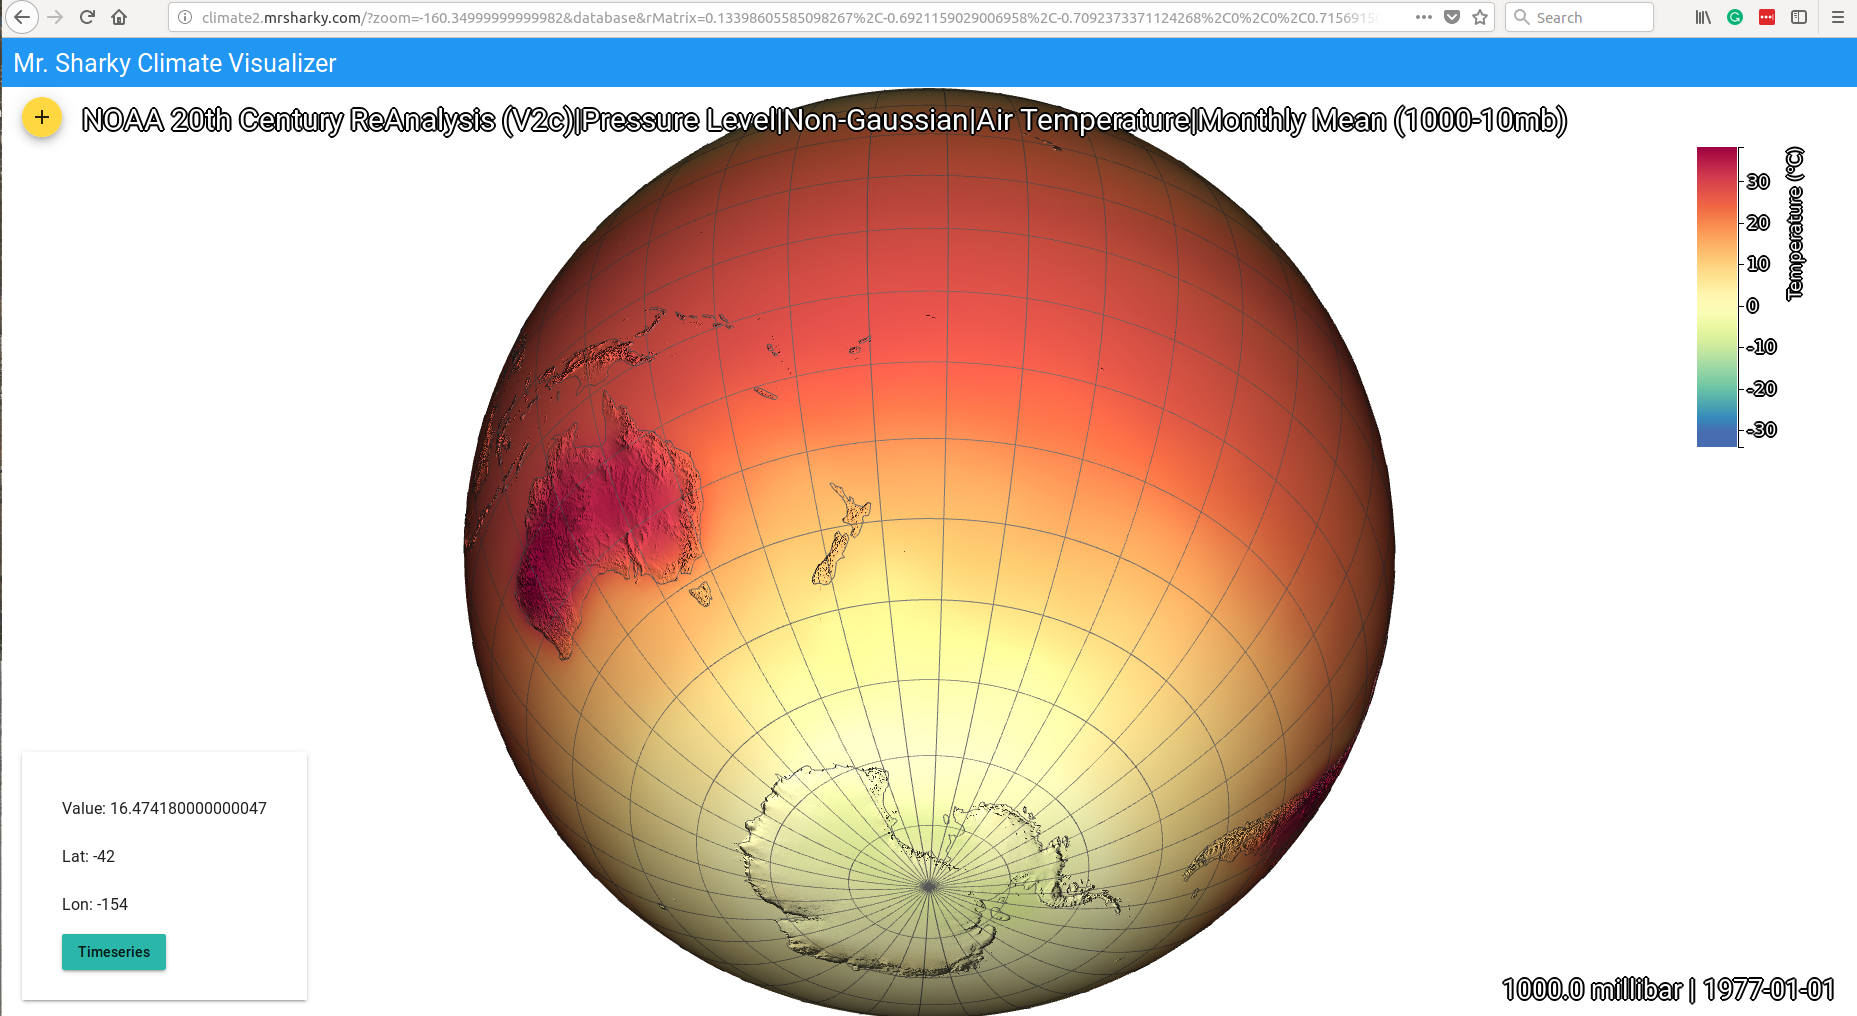
\includegraphics[width=.75\linewidth]{mrSharkySouthView.png}}
\fbox{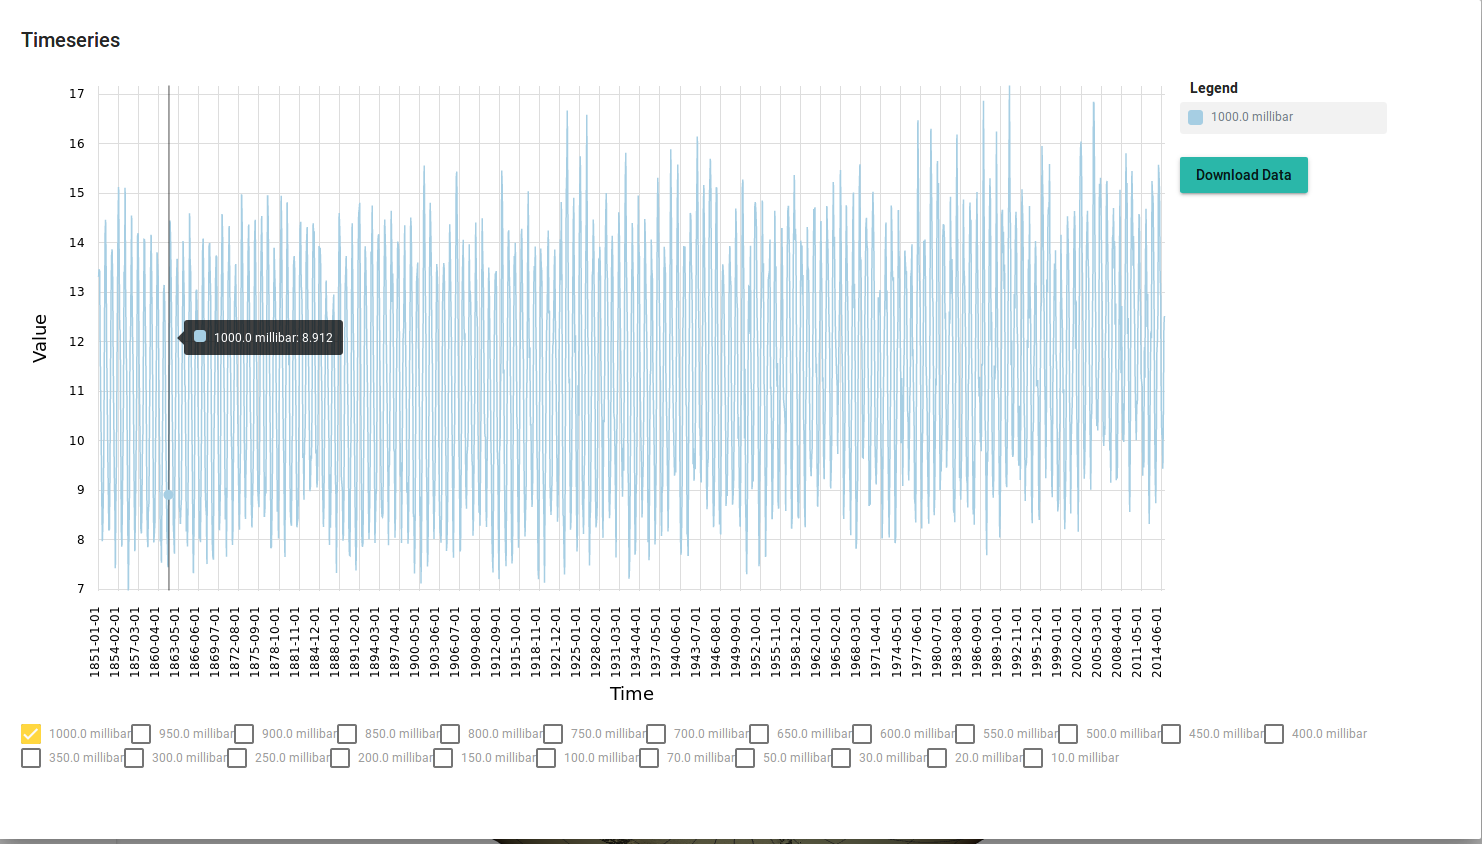
\includegraphics[width=.75\linewidth]{mrShTS.png}}
\caption{\label{fig:mr_sh_south} Clicking a point on the globe will generate a box element showing the point's value and latitude-longitude coordinates, shown in the lower left corner of the (top) subfigure. Clicking the teal button will generate a time series (bottom) that can be downloaded as a .csv file.}
\end{minipage}
\end{figure}

This app is intuitive enough to use, yet allows a great deal of customization. The sidebar control lets users select different projections, datasets, color bars, adjust sphere resolution, et cetera.

The bulk of the server side involves the transfer of HTML scripts and data\cite{pierret20174d}. Pushing the plotting, rastering, and graphics manipulation tasks to the client side unburden the server, reducing the hardware and networking resource requirements and lowering the cost to run the app. 

MrSharky's architecture and data delivery method has influenced the web app described in Section~\ref{argovis} and in Chapter 3 of this thesis.

\subsection{Visualization and data retrieval tool Argovis} \label{argovis}

This thesis introduces a new website at \url{www.argovis.com} that allows easy navigation of profiles from the Argo GDACs. This web app offers a simple user interface and allows both scientists and the general public to draw polygons on an interactive map and view the profiles within given date and depth ranges. After selection, the user may browse T/S/P profiles on interactive charts, either from a single float or those found within the drawn polygons. Some metadata about the floats are displayed as well, along with a list of links to locate the data of interest on the GDACs.

Overall, Argovis offers seamless navigation of the Argo dataset written with a representational state transfer (REST) architecture. RESTful design allows the opportunity to feature API and cloud computing applications, e.g., map comparison from existing gridded Argo products, as well as derived variables. Argo now has a maintainable, scalable, and portable tool to support this ever-expanding big data set. Chapter 3 shall provide further detail on the web app's front end and back end architecture and database information, along with some time series and grid-interpolation applications.